\begin{sol}
\begin{enumerate}[label=\textbf{(\alph*)}]
    \item For $b=0$, we have the finite square well where the wavefunction is sinusoidal inside and exponentially decaying outside.
    \vspace{2mm}
    
    For $b=a$, we have the double square well problem similar to question 6 on problem set 6, where we have drawn what the first even solution looks like. The first odd solution will look like:
    \begin{center}
        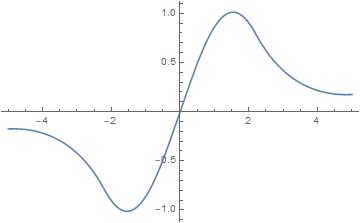
\includegraphics[width=0.5\linewidth]{Images/7-2a.png}
    \end{center}
    \vspace{2mm}
    
    For $b \gg a$, we have a similar situation except the two wells will be not affected (or very little) by each other. Outside the wells, the wavefunction quickly goes to near zero.
    
    \item As discussed, it makes sense for the energies of both even and odd states to approach the same value $V_0$ as the separation $b$ goes to infinity. The first even state has a negative energy so its energy starts below $V_0$. The first odd state has a positive energy so its total energy starts above $V_0$. Thus $E_1$ is monotonically increasing while $E_2$ is monotonically decreasing.
    
    \item Since systems tend to seek a lower energy level, so an electron in the even state tends to draw the protons together and an electron in the odd state does the opposite.
\end{enumerate}
\end{sol}